
\documentclass[addpoints]{exam}
% Used to insert images
\usepackage{graphicx}
\usepackage{color}

% \printanswers

\newcommand{\event}{Kinematics}
\def\type{0}

\setlength\fillinlinelength{\textwidth}
\CorrectChoiceEmphasis{\color{red}\bfseries}
\SolutionEmphasis{\color{red}\bfseries}

\setlength\answerclearance{2pt}
\pagestyle{headandfoot}
% Adds a line to the top of the page
\runningheadrule
% The three braces correspond to the different parts of the header: the left is the top left text, middle is top middle, and right is top right.
\runningheader{\event}{\tournament}{\ifnum\type=1 Class Set Test \else Full Name:\hspace{1cm} \fi }
% Adds a line to the bottom of the page
\runningfootrule
% The three braces correspond to the different parts of the footer: the left is the bottom left text, middle is bottom middle, and right is bottom right.
% Doesn't include the title page in the page count 
% \runningfooter{}{Page \the\numexpr\thepage-1\   of \the\numexpr\numpages-1}{}
% Uncomment the line below if you want to include the title page in the page count 
\runningfooter{}{Page \thepage\   of \numpages}{}

\begin{document}
\begin{center}
    {\huge Grade 12 Physics \\ \event
    % Writes key if the answers are shown, otherwise writes test
    \ifprintanswers 
     \space Key
    \else 
     \space \ifnum\type<2 Test \fi \ifnum\type=1 \textbf{(CLASS SET)} \fi \ifnum\type=2 Answer Sheet \fi
    \fi \\ \vspace{3mm}\tournament\vspace{1mm}}
\end{center}
% Change to any picture or just some \vspace{.3\textheight} to leave it blank. [h] ensures that the image is placed in the same place in the document as in the code
\begin{figure}[h]
    \centering
    \includegraphics[height=.3\textheight, width=.6\textwidth, keepaspectratio]{}
\begin{figure}
    \centering
    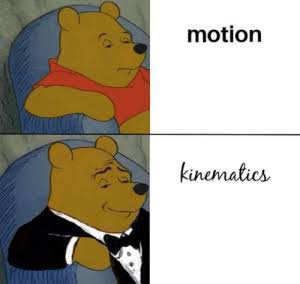
\includegraphics[width=0.5\linewidth]{winnie-the-pooh-kinematics.jpg}
    \label{fig:enter-label}
\end{figure}
\end{figure}


\begin{center}
    First Name: \ifprintanswers
    \underline{\hspace{3.5cm}}\textbf{KEY}\underline{\hspace{5.5cm}}\\\vspace{5mm}
    \else
        \underline{\hspace{10cm}}\\ \vspace{5mm}
    \fi
    Last Name: \underline{\hspace{10cm}}\\ \vspace{5mm}

\end{center}

% Change the list below to reflect the instructions for your test
\noindent\textbf{\underline{Directions:}}
\begin{itemize}
    % If the test is a class set, an instruction will appear to not write on the test paper.
    \ifnum\type=1 \item \textbf{This test is a class set.} Please do not write any answers on this paper. \fi
    % Adds an instruction 
    \item Please answer to 2 decimal points
    \item The test is designed to be completed in 75 minutes
\end{itemize}
\begin{center}
\textit{For grading use only}\\
% The gradetable has a number of rows that automatically updates. This is not very accurate because of the variance in question size, but it can serve as a starting point. You will probably need to manually update the number of rows of the gradetable (change '\the\numexpr\numpages/13+1' to the desired number of rows).
\multirowgradetable{1}[pages]   
\end{center}

\newpage
\begin{questions}

\section*{Questions}

\question[1] A car accelerates uniformly from rest to a speed of 25 m/s in 10 seconds. What is the car's acceleration?
\begin{choices}
    \choice 1.5 m/s$^2$
    \correctchoice 2.5 m/s$^2$
    \choice 3.5 m/s$^2$
    \choice 4.5 m/s$^2$
\end{choices}

\question[1] An object is thrown vertically upward with an initial velocity of 20 m/s. What is its velocity after 3 seconds? (Assume $g = 9.8$ m/s$^2$.)
\begin{choices}
    \choice 10.6 m/s
    \choice 0 m/s
    \correctchoice -9.4 m/s
    \choice -19.4 m/s
\end{choices}

\question[1] A ball is dropped from a height of 80 m. How long does it take to hit the ground? (Assume $g = 9.8$ m/s$^2$.)
\begin{choices}
    \correctchoice 4 s
    \choice 5 s
    \choice 6 s
    \choice 7 s
\end{choices}

\question[1] A car traveling at 20 m/s comes to a stop in 4 seconds. What is the magnitude of its acceleration?
\begin{choices}
    \choice 4 m/s$^2$
    \correctchoice 5 m/s$^2$
    \choice 6 m/s$^2$
    \choice 7 m/s$^2$
\end{choices}

\question[1] An object moves with a constant velocity of 15 m/s for 10 seconds. What is its displacement?
\begin{choices}
    \choice 100 m
    \choice 125 m
    \correctchoice 150 m
    \choice 200 m
\end{choices}

\question[1] A ball is thrown upward with a velocity of 30 m/s. How long does it take to reach the maximum height? (Assume $g = 9.8$ m/s$^2$.)
\begin{choices}
    \choice 2.5 s
    \correctchoice 3.0 s
    \choice 3.5 s
    \choice 4.0 s
\end{choices}

\question[1] A cyclist accelerates uniformly from rest to a velocity of 10 m/s in 5 seconds. What is the total distance covered during this time?
\begin{choices}
    \choice 15 m
    \choice 20 m
    \correctchoice 25 m
    \choice 30 m
\end{choices}


\question[1] An object accelerates uniformly at 4 m/s$^2$ for 6 seconds. If it starts from rest, what is its final velocity?
\begin{choices}
    \choice 20 m/s
    \correctchoice 24 m/s
    \choice 28 m/s
    \choice 32 m/s
\end{choices}

\question[1] A rock is thrown horizontally at 15 m/s from a cliff that is 45 m high. How long does it take for the rock to hit the ground? (Assume $g = 9.8$ m/s$^2$.)
\begin{choices}
    \choice 2.5 s
    \correctchoice 3.0 s
    \choice 3.5 s
    \choice 4.0 s
\end{choices}

\question[1] A ball is thrown downward with an initial velocity of 5 m/s. How far does it fall in 3 seconds? (Assume $g = 9.8$ m/s$^2$.)
\begin{choices}
    \choice 35.4 m
    \correctchoice 44.1 m
    \choice 53.4 m
    \choice 62.1 m
\end{choices}

\question[1] A ball is dropped from rest, and after falling for 3 seconds, its velocity is:
\begin{choices}
\choice 9.8 m/s
\correctchoice 19.6 m/s
\choice 29.4 m/s
\choice 39.2 m/s
\end{choices}

\question[1] A train is traveling at 40 m/s and slows down uniformly to 20 m/s over 10 seconds. What is the distance traveled during this time?
\begin{choices}
\choice 100 m
\correctchoice 200 m
\choice 300 m
\choice 400 m
\end{choices}

\question[1] A projectile is launched at an angle of 45° with an initial velocity of 50 m/s. What is the total time of flight? (Assume $g = 9.8$ m/s$^2$.)
\begin{choices}
\correctchoice 7.1 s
\choice 8.2 s
\choice 9.3 s
\choice 10.2 s
\end{choices}

\question[1] A car is traveling at 30 m/s and accelerates uniformly at 3 m/s$^2$. How long does it take to reach a velocity of 60 m/s?
\begin{choices}
\choice 5 s
\choice 10 s
\correctchoice 15 s
\choice 20 s
\end{choices}

\question[1] An object is thrown vertically upward with an initial velocity of 15 m/s. What is its maximum height? (Assume $g = 9.8$ m/s$^2$.)
\begin{choices}
\choice 8.6 m
\choice 10.2 m
\correctchoice 11.5 m
\choice 12.8 m
\end{choices}


\question[1] A car accelerates uniformly from 10 m/s to 30 m/s over a distance of 100 m. What is the car’s acceleration?
\begin{choices}
\choice 2 m/s$^2$
\choice 3 m/s$^2$
\correctchoice 4 m/s$^2$
\choice 5 m/s$^2$
\end{choices}

\question[1] An object is projected horizontally from a height of 80 m with a velocity of 20 m/s. How far does it travel horizontally before hitting the ground? (Assume $g = 9.8$ m/s$^2$.)
\begin{choices}
\choice 80 m
\choice 100 m
\correctchoice 120 m
\choice 160 m
\end{choices}

\question[1] A ball is thrown downward with an initial velocity of 10 m/s. After 4 seconds, its velocity is:
\begin{choices}
\choice 29.8 m/s
\choice 39.2 m/s
\correctchoice 49.6 m/s
\choice 59.0 m/s
\end{choices}

\question[1] A cyclist travels 20 m at 4 m/s, then another 30 m at 6 m/s. What is their average velocity?
\begin{choices}
\choice 4.8 m/s
\choice 5.0 m/s
\correctchoice 5.2 m/s
\choice 5.4 m/s
\end{choices}

\question[1] A rocket accelerates from rest at 10 m/s$^2$ for 12 seconds. What is its final velocity?
\begin{choices}
\correctchoice 100 m/s
\choice 110 m/s
\choice 120 m/s
\choice 130 m/s
\end{choices}



\section*{Short Answer}

\question[5] Derive the kinematic equation $v^2 = u^2 + 2as$ using basic definitions of acceleration and displacement.?
\begin{solution}[6cm]
    To derive the equation \(v^2 = u^2 + 2as\), we start with the following basic kinematic definitions:
\begin{itemize}
    \item Acceleration (\(a\)) is defined as the rate of change of velocity:
    \[
    a = \frac{v - u}{t}, \quad \text{where } u \text{ is the initial velocity, } v \text{ is the final velocity, and } t \text{ is the time.}
    \]
    Rearranging, we get:
    \[    v = u + at. \quad \text{(Equation 1)}\]
    \item Displacement (\(s\)) is given by:
    \[    s = ut + \frac{1}{2}at^2. \quad \text{(Equation 2)}\]
\end{itemize}
Substitute \(t = \frac{v - u}{a}\) (from Equation 1) into Equation 2:
\[
s = u\left(\frac{v - u}{a}\right) + \frac{1}{2}a\left(\frac{v - u}{a}\right)^2.
\]
Simplify each term:
\[
s = \frac{u(v - u)}{a} + \frac{1}{2}a\frac{(v - u)^2}{a^2}.
\]
\[s = \frac{u(v - u)}{a} + \frac{(v - u)^2}{2a}.\]
Combine the terms under a common denominator:
\[s = \frac{2u(v - u) + (v - u)^2}{2a}.\]
Expand and simplify the numerator:
\[s = \frac{v^2 - u^2}{2a}.\]
Finally, rearrange to isolate \(v^2\):
\[v^2 = u^2 + 2as.\]
\end{solution}



\question A train moves with a constant acceleration of 2 m/s$^2$ for 15 seconds. If it starts from rest, calculate:
\begin{parts}
    \part[2] The acceleration
    \part[3] The distance traveled during this time.
\end{parts}
\begin{solution}[5cm]
    Given:
\begin{itemize}
    \item Acceleration, \(a = 2 \, \mathrm{m/s^2}\),
    \item Time, \(t = 15 \, \mathrm{s}\),
    \item Initial velocity, \(u = 0 \, \mathrm{m/s}\).
\end{itemize}

(a) The acceleration is already given as:
\[a = 2 \, \mathrm{m/s^2}.\]

(b) The distance traveled (\(s\)) can be calculated using the equation:
\[s = ut + \frac{1}{2}at^2.\]
Substitute the given values:
\[s = (0)(15) + \frac{1}{2}(2)(15)^2,\]
\[s = 0 + \frac{1}{2}(2)(225),\]
\[s = 225 \, \mathrm{m}.\]

\textbf{Final answers:}
\begin{itemize}
    \item (a) The acceleration is \(2 \, \mathrm{m/s^2}\).
    \item (b) The distance traveled is \(225 \, \mathrm{m}\).
\end{itemize}
\end{solution}



\question A rocket is launched vertically upward with an initial velocity of 50 m/s. Calculate:
\begin{parts}
    \part[2] The maximum height it reaches.
    \part[3] The total time it takes to return to the ground.
\end{parts}
\begin{solution}[5cm]
    Given:
\begin{itemize}
    \item Initial velocity, \(u = 50 \, \mathrm{m/s}\),
    \item Acceleration due to gravity, \(a = -9.8 \, \mathrm{m/s^2}\).
\end{itemize}

(a) To calculate the maximum height (\(h\)), we use the kinematic equation:
\[v^2 = u^2 + 2as,\]
where \(v = 0 \, \mathrm{m/s}\) at the maximum height.

Substitute the values:
\[0 = (50)^2 + 2(-9.8)h,\]
\[0 = 2500 - 19.6h,\]
\[h = \frac{2500}{19.6} \approx 127.55 \, \mathrm{m}.\]

(b) To calculate the total time (\(t\)) it takes to return to the ground, we first find the time to reach the maximum height:
\[v = u + at.\]
Substitute the values:
\[0 = 50 + (-9.8)t,\]
\[t = \frac{50}{9.8} \approx 5.10 \, \mathrm{s}.\]
The total time to return to the ground is twice the time to reach the maximum height:
\[t_{\text{total}} = 2 \times 5.10 \approx 10.20 \, \mathrm{s}.\]

\textbf{Final answers:}
\begin{itemize}
    \item (a) The maximum height is approximately \(127.55 \, \mathrm{m}\).
    \item (b) The total time to return to the ground is approximately \(10.20 \, \mathrm{s}\).
\end{itemize}

\end{solution}



\question Two cars start from rest at the same point. Car A accelerates uniformly at 3 m/s$^2$, while Car B accelerates uniformly at 2 m/s$^2$. Calculate:
\begin{parts}
    \part[2] The time it takes for Car A to be 30 m ahead of Car B.
    \part[3] The distance covered by each car at this time.
\end{parts}
\begin{solution}[6cm]
Given:
\begin{itemize}
    \item Acceleration of Car A, \(a_A = 3 \, \mathrm{m/s^2}\),
    \item Acceleration of Car B, \(a_B = 2 \, \mathrm{m/s^2}\),
    \item Both cars start from rest (\(u_A = u_B = 0 \, \mathrm{m/s}\)).
\end{itemize}

(a) To find the time (\(t\)) it takes for Car A to be 30 m ahead of Car B, we calculate the displacement of each car using:
\[s = ut + \frac{1}{2}at^2.\]
The displacement of Car A is:
\[s_A = \frac{1}{2}a_A t^2 = \frac{1}{2}(3)t^2 = 1.5t^2.\]
The displacement of Car B is:
\[s_B = \frac{1}{2}a_B t^2 = \frac{1}{2}(2)t^2 = t^2.\]
The condition is:
\[s_A - s_B = 30,\]
\[1.5t^2 - t^2 = 30,\]
\[0.5t^2 = 30,\]
\[t^2 = 60 \implies t = \sqrt{60} \approx 7.75 \, \mathrm{s}.\]

(b) To find the distance covered by each car at this time:
\[s_A = 1.5t^2 = 1.5(60) = 90 \, \mathrm{m},\]
\[s_B = t^2 = 60 \, \mathrm{m}.\]

\textbf{Final answers:}
\begin{itemize}
    \item (a) The time it takes for Car A to be 30 m ahead of Car B is approximately \(7.75 \, \mathrm{s}\).
    \item (b) The distance covered by Car A is \(90 \, \mathrm{m}\), and by Car B is \(60 \, \mathrm{m}\).
\end{itemize}
\end{solution}



\question A ball is thrown vertically upward with an initial velocity of 25 m/s. After 2 seconds, another ball is thrown upward with the same velocity. Determine:
\begin{parts}
    \part[5] The time at which the two balls meet.
    \part[5] The height at which they meet.
\end{parts}
\begin{solution}[8cm]
    \textbf{Given:}
\begin{itemize}
    \item Initial velocity of both balls, \(u = 25 \, \mathrm{m/s}\),
    \item Acceleration due to gravity, \(a = -9.8 \, \mathrm{m/s^2}\),
    \item Second ball is thrown \(t = 2 \, \mathrm{s}\) after the first ball.
\end{itemize}

\textbf{Solution:}

(a) Let the time after the first ball is thrown at which they meet be \(t_1\) (for the first ball). 

For the first ball, its position \(y_1\) is given by:
\[
y_1 = ut_1 + \frac{1}{2}at_1^2.
\]
Substituting the known values:
\[
y_1 = 25t_1 - 4.9t_1^2.
\]

For the second ball, let its position \(y_2\) be expressed relative to the time it was thrown. It is thrown 2 seconds after the first ball, so its time of motion is \(t_1 - 2\). Its position is:
\[
y_2 = u(t_1 - 2) + \frac{1}{2}a(t_1 - 2)^2.
\]
Substituting the known values:
\[
y_2 = 25(t_1 - 2) - 4.9(t_1 - 2)^2.
\]

The balls meet when \(y_1 = y_2\):
\[
25t_1 - 4.9t_1^2 = 25(t_1 - 2) - 4.9(t_1 - 2)^2.
\]

Expanding and simplifying:
\[
25t_1 - 4.9t_1^2 = 25t_1 - 50 - 4.9(t_1^2 - 4t_1 + 4).
\]
\[
25t_1 - 4.9t_1^2 = 25t_1 - 50 - 4.9t_1^2 + 19.6t_1 - 19.6.
\]
\[
0 = -50 - 19.6 + 19.6t_1.
\]
\[
19.6t_1 = 69.6 \implies t_1 = \frac{69.6}{19.6} \approx 3.55 \, \mathrm{s}.
\]

The second ball's time of motion is:
\[
t_2 = t_1 - 2 = 3.55 - 2 = 1.55 \, \mathrm{s}.
\]

(b) To find the height at which they meet, substitute \(t_1 = 3.55 \, \mathrm{s}\) into the equation for \(y_1\):
\[
y_1 = 25(3.55) - 4.9(3.55)^2.
\]
\[
y_1 = 88.75 - 61.63 \approx 27.12 \, \mathrm{m}.
\]

\textbf{Final answers:}
\begin{itemize}
    \item (a) The two balls meet at approximately \(t = 3.55 \, \mathrm{s}\) after the first ball is thrown.
    \item (b) The height at which they meet is approximately \(27.12 \, \mathrm{m}\).
\end{itemize}
\end{solution}



\question A cyclist starts from rest and accelerates uniformly at a rate of 1.5 m/s$^2$ for 12 seconds. She then maintains a constant velocity for 20 seconds before decelerating uniformly to rest in 8 seconds.
\begin{parts}
    \part[3] Draw a velocity-time graph for the motion.
    \part[3] Calculate the total distance traveled.
    \part[4] Calculate the average velocity for the entire trip.
\end{parts}
\begin{solution}[7cm]
    \textbf{Given:}
\begin{itemize}
    \item Acceleration \(a_1 = 1.5 \, \mathrm{m/s^2}\),
    \item Time of acceleration \(t_1 = 12 \, \mathrm{s}\),
    \item Constant velocity time \(t_2 = 20 \, \mathrm{s}\),
    \item Deceleration time \(t_3 = 8 \, \mathrm{s}\).
\end{itemize}

\textbf{Solution:}

(a) The velocity-time graph can be drawn as follows:
The cyclist accelerates uniformly for 12 seconds, reaching a velocity:
\[
v_{\text{max}} = a_1 \cdot t_1 = 1.5 \cdot 12 = 18 \, \mathrm{m/s}.
\]
She then maintains this constant velocity for 20 seconds, before decelerating uniformly to rest over 8 seconds.

The graph consists of three segments:
\begin{itemize}
    \item A linearly increasing segment from \(0\) to \(18 \, \mathrm{m/s}\) over \(12 \, \mathrm{s}\),
    \item A horizontal segment at \(18 \, \mathrm{m/s}\) for \(20 \, \mathrm{s}\),
    \item A linearly decreasing segment from \(18 \, \mathrm{m/s}\) to \(0\) over \(8 \, \mathrm{s}\).
\end{itemize}

(b) The total distance traveled is the area under the velocity-time graph. The graph forms a trapezoid:
\[
\text{Total distance} = \text{Area of trapezoid}.
\]
\[
\text{Distance} = \frac{1}{2} \cdot (\text{Base}_1 + \text{Base}_2) \cdot \text{Height}.
\]

For the three segments:
\[
\text{Distance during acceleration} = \frac{1}{2} \cdot 12 \cdot 18 = 108 \, \mathrm{m}.
\]
\[
\text{Distance during constant velocity} = 18 \cdot 20 = 360 \, \mathrm{m}.
\]
\[
\text{Distance during deceleration} = \frac{1}{2} \cdot 8 \cdot 18 = 72 \, \mathrm{m}.
\]

Total distance:
\[
\text{Total distance} = 108 + 360 + 72 = 540 \, \mathrm{m}.
\]

(c) To find the average velocity, use:
\[
v_{\text{avg}} = \frac{\text{Total distance}}{\text{Total time}}.
\]
\[
\text{Total time} = 12 + 20 + 8 = 40 \, \mathrm{s}.
\]
\[
v_{\text{avg}} = \frac{540}{40} = 13.5 \, \mathrm{m/s}.
\]

\textbf{Final answers:}
\begin{itemize}
    \item (a) The velocity-time graph consists of a linear increase, a constant segment, and a linear decrease.
    \item (b) The total distance traveled is \(540 \, \mathrm{m}\).
    \item (c) The average velocity for the entire trip is \(13.5 \, \mathrm{m/s}\).
\end{itemize}
\end{solution}



\question A ball is dropped from a height of 200 m. At the same instant, another ball is thrown upward from the ground with an initial velocity of 50 m/s. Determine:
\begin{parts}
    \part[3] The time at which the two balls meet.
    \part[4] The height at which they meet.
    \part[3] The velocities of both balls at the point of meeting.
\end{parts}
\begin{solution}[12cm]
    \textbf{(a) The time at which the two balls meet:}

Using the equations of motion for the two balls:  
For the first ball (dropped from 200 m):  
\[
y_1 = 200 - \frac{1}{2} g t^2
\]  
For the second ball (thrown upward):  
\[
y_2 = v_0 t - \frac{1}{2} g t^2
\]  
Equating \(y_1 = y_2\):  
\[
200 - \frac{1}{2} g t^2 = v_0 t - \frac{1}{2} g t^2
\]  
Simplifying:  
\[
200 = v_0 t
\]  
\[
t = \frac{200}{v_0} = \frac{200}{50} = 4 \, \text{seconds.}
\]

\textbf{(b) The height at which the two balls meet:}

Substitute \(t = 4\) into \(y_2\):  
\[
y = v_0 t - \frac{1}{2} g t^2 = 50(4) - \frac{1}{2}(9.8)(4)^2
\]  
\[
y = 200 - 78.4 = 121.6 \, \text{meters.}
\]

\textbf{(c) The velocities of both balls at the point of meeting:}

For the first ball:  
\[
v_1 = -g t = -(9.8)(4) = -39.2 \, \text{m/s.}
\]  
For the second ball:  
\[
v_2 = v_0 - g t = 50 - (9.8)(4) = 50 - 39.2 = 10.8 \, \text{m/s.}
\]
\end{solution}



\question A car moving at 25 m/s decelerates uniformly to a stop over a distance of 100 m. It then reverses direction, accelerating uniformly at 2 m/s$^2$ until it reaches a velocity of 20 m/s. Calculate:
\begin{parts}
    \part[2] The time taken to stop.
    \part[4] The time taken to reach 20 m/s in reverse.
    \part[4] The total distance covered by the car.
\end{parts}
\begin{solution}[5cm]
    \textbf{(a) The time taken to stop:}

Using \(v^2 = u^2 + 2as\):  
\[
0 = 25^2 + 2(-a)(100)
\]  
\[
625 = 200a \quad \Rightarrow \quad a = -3.125 \, \text{m/s}^2
\]  
\[
t = \frac{v - u}{a} = \frac{0 - 25}{-3.125} = 8 \, \text{seconds.}
\]

\textbf{(b) The time taken to reach 20 m/s in reverse:}

Using \(v = u + at\):  
\[
t = \frac{v - u}{a} = \frac{20 - 0}{2} = 10 \, \text{seconds.}
\]

\textbf{(c) The total distance covered by the car:}

First phase (deceleration):  
\[
s_1 = \frac{1}{2} (u + v) t = \frac{1}{2} (25 + 0)(8) = 100 \, \text{meters.}
\]  

Second phase (reverse motion):  
\[
s_2 = \frac{1}{2} (u + v) t = \frac{1}{2} (0 + 20)(10) = 100 \, \text{meters.}
\]  

Total distance:  
\[
s = s_1 + s_2 = 100 + 100 = 200 \, \text{meters.}
\]
\end{solution}


\end{questions}

\end{document}
